\section{Quality control and processing} \label{processing}
\subsection{Verification of input data and conversion to a common data model}\label{format-check}
The source data for ICOADS is stored in the fixed width International Maritime Meteorological Archive (IMMA) format (see \url{https://icoads.noaa.gov/doc.html}). 
This format consists of one weather report per record with a core data section and optional attachments containing additional information.
Table \ref{tab:imma_structure} summarises the different attachments, those in italic are typically reported with each report regardless of source. 
The presence of the other attachments depends on both on the type of platform / station making the weather report and the source of the data. 
For example, the IMMT attachment will only be present for ship observations.

Prior to converting to the common data model, used by the C3S service for both land and marine data, the individual ICOADS records are checked against the specification of the IMMA format. 
Each element in IMMA has a defined data type and valid range. 
Similarly, valid enumerated (or coded) values are specified via a code table.
Any record with an element falling outside the specified valid range, with the exception of missing data, or with an invalid coded value is discarded.
Similarly, reports with an invalid date, time or location are discarded from further processing. No QC flags are set.
After validation, the IMMA records are converted to the common data model (see Section \ref{data_model}) and the quality control described below applied.

\begin{table}
\centering
\caption{Sections of an IMMA record (see \url{https://icoads.noaa.gov/doc.html} for a full description)}
\label{tab:imma_structure}
%\begin{center}
\begin{tabular}{|p{0.2\linewidth}|p{0.2\linewidth}|p{0.5\linewidth}|}
\hline
\bfseries Attachment name & \bfseries Abbreviation & \bfseries Description \\
\hline
\it Core & Core & ICOADS core record containing commonly observed parameters, date and time\\\hline
\it ICOADS attachment & ICOADS & Attachment containing ship/ platform identification, additional observed parameters and ICOADS QC flags \\\hline
IMMT-5 / FM 13 attachment & IMMT & Attachment containing additional information reported by Voluntary Observing Ships in either the International Marine Meteorological Tape (IMMT) or WMO FM-13 formats. \\\hline
Model QC attachment & Mod-QC & Attachment containing NWP model data collocated to the location the observations. \\\hline
Ship metadata attachment & Meta-VOS & Attachment containing limited metadata from WMO-No. 47 merged with ship observations in ICOADS. \\\hline
Near surface oceanographic data attachment & NOcn & Attachment containing surface ocean biogeochemical measurements \\\hline
Edited cloud report & ECR & Attachment containing corrected / edited cloud observations following Hahn and Warren (1999). \\\hline
Reanalysis QC / feedback attachment & Rean-QC & Attachment providing the facility to include observation feedback information from reanalysis models \\\hline
IVAD attachment & IVAD & Attachment to store data from the ICOADS Value Added Database Project \\\hline
Error attachment & Error & Attachment designed to support the correction of erroneous IMMA elements. \\\hline
\it Unique report ID attachment & UIDA & Attachment with unique ID assigned to each report \\\hline
\it Supplemental data attachment & Suppl. & Attachment to store additional data not representable in other attachments and to store the weather reports in the orignal format / units where available. The format of the Suppl. attachment is source and deck dependent.\\\hline
\end{tabular}
%\end{center}
\end{table}


\subsection{Station/platform identification (ship only)}
The station / platform identification within ICOADS is stored in the ID field and over the lifetime of the marine meteorological observations and archives a wide variety of formats have been used to identify individual ships. 
For example, in the early punchcard decks from the 1960s and earlier, ships were assigned a numeric identifier allocated in alphabetical order each year with the ship names written on the back of the punchcard. Lists matching the ship numbers to ship names were created and archived. 
However, over time and with the conversion from punchcards to magnetic tape and then to digital formats the link between ships names and numbers have been lost, with only the ship number remaining.
For some decks the ship number has subsequently been dropped where it was thought to have no value without the link to the ship name.
In other cases the logbook number was used to identify the digitised data, sometimes with a page number appended.
More recently, ship names or abbreviated ship names have been recorded directly in the digitised data when logbooks have been keyed.
For realtime data sources we typically have the ITU callsign or a masked/generic identifier.
Overall, there are many sources of error and ambiguity in the station / platform identification field.
These issues are discussed further in \cite{Carella2017_tracking} and we follow the method of \cite{Carella2017_tracking} to link observations from the same ship together.
As part of this process the ID field has been corrected for known errors and new ids assigned where the ID field is missing, a generic ID assigned or set to a logbook and page number.

\subsection{Duplicate detection and flagging (ship only)} \label{ship-dupelim}
Duplicates exist in ICOADS due to the way that the dataset has been created over many decades with data from many different sources, often with overlapping observations, merged. 
For example, many national climate archives such as those in the US, UK, Germany and Netherlands were based on the same source data with the ship logbooks digitised once and then shared between nations. 
This process has been repeated several times resulting in many duplicates in the underpinning data. 
For recent decades multiple realtime GTS sources have been ingested as this has been shown to increase the number of unique reports but at the expense of increased duplicates. 
Similarly, when the higher quality delayed mode versions of the real time data are ingested the real time versions need to be flagged and replaced. 
As part of the processing to create ICOADS the duplicate detection and elimination software (DUPELIM) is run, with only those reports believed to be unique released into the final versions (e.g. see \cite{Freeman2017}, \cite{Woodruff2011})\footnote{additional information is also available from https://icoads.noaa.gov/dupelim.html}.

The ICOADS DUPELIM software relies heavily on the date, time, location and station / platform identification. 
All of these fields may contain errors due to a number of reasons. 
For example, an observation may be mis-assigned to the wrong day or an observation put in the wrong location due to the mis-coding of the quadrant of the globe within the data records when the data were originally keyed. 
In other cases, the data have been modified or stored differently in the different archives.
For example, the location of an observation was often recorded as the one degree latitude / longitude grid box the observation was located in.
On conversion to a latitude / longitude pair the location could be given either as the edge of the grid box or the grid box center, resulting in different locations for the same observation.
Conversion between units and the enumeration / translation between code tables can also introduce minor differences.
As such, due to those differences not all duplicates have been identified by the DUPELIM software and unidentified duplicates exist in the ICOADS final files.

Within the C3S service an additional level of duplicate detection has been performed making allowances for these known issues.
In many cases the results are similar to that of DUPELIM but with an increase of up to 5 - 10 \% in the number of duplicates identified in some periods.
The method and results are fully described in \cite{Kent2019dup}, table \ref{tab:dup_flags} lists the categorisations used.

\begin{table}
\centering
\caption{Duplicate flags and meanings used within the common data model (see Section )}
\label{tab:dup_flags}
%\begin{center}
\begin{tabular}{|p{0.1\linewidth}|p{0.3\linewidth}|p{0.5\linewidth}|}
\hline
\bfseries Flag value & \bfseries Meaning & \bfseries Comments \\
\hline
0 & Unique observation, no known duplicates & \\\hline
1 & Best duplicate & \\\hline
2 & Duplicate & This has been used to identify reports thought to be duplicates but where no selection was made, e.g. because there were unique variables present in each report. \\\hline
3 & Worst duplicate & \\\hline
4 & Unchecked & Reports have not been through the duplicate elimination process.\\\hline
\end{tabular}
%\end{center}
\end{table}


\subsection{Drifting buoy identification and duplicate flagging}\label{buoy-dupelim}
Due to the different data management practices and data streams for the drifting buoy data compared to ships many of the issues present in the ship data are avoided. 
The prevalence of mis-coding errors in the date, time, location and buoy ID fields is thought to be negligible.
As such, within the C3S service we make use of the ICOADS intermediate reject flag (IRF) to identify the best duplicates to keep.
Drifting buoy reports with IRF set to \texttt{retain} have their report quality flag within the common data model set to 0 (pass).
All other buoy reports have their report quality flag set to 1 (failed). 
In all cases, the duplicate flag is set to 4 (unchecked).

\subsection{Advanced quality control}
Once the observations have been through the initial format checks, station / platform identification and duplicate flagging three additional stages of quality control are performed. 
These are based on a scheme developed by the UK Met Office and described in \cite{Kennedy2017} and repeated here for completeness.
Prior to proceeding to the advanced quality control some pre-screening is performed.
For a ship based report to proceed to the advanced quality control stage it needs to have been flagged as either the best duplicate or a unique report (section \ref{ship-dupelim}).
For a buoy based report to proceed it needs to have been flagged for retention by the ICOADS IRF flag and initially marked as passing the report quality check (section \ref{buoy-dupelim}).
All other observations have their report and observation quality flags set to unchecked. No additional quality control data will be generated for these reports.

\subsubsection{Report level quality control} \label{report-qc}
The report level quality control checks are similar to those performed as part of the verification of input data (section \ref{format-check}).
Three different flags are set based on the validity of the date, time and location of a report. 1 indicates a fail and 0 a pass.
In addition to these checks the station / platform identifier is checked against a list of those stations known to produce low quality data (see Table \ref{tab:blacklist}). 
Observations with a station / platform identifier matching one on the list have their black list flag set to 1. All others are set to zero.
The flags are:
\begin{enumerate}
\item \texttt{Time check}: Check whether time of observation is valid (0 $\leq$ hour $\leq$ 24). 1 returned for invalid or missing times, 0 otherwise.
\item \texttt{Date check}: Check whether date is valid and in the range 1850 to 2024. 1 returned for invalid dates or dates outside the specified range, 0 otherwise.
\item \texttt{Location check}: Check whether location (latitude and longitude) is valid. 1 returned for latitude outside the range 90 S to 90 or for longitude outside the range 180W to 360E. 1 also returned for missing data, 0 returned in all other cases.
\item \texttt{Blacklist}: Flag set to 1 for any observation matching a condition listed in table \ref{tab:blacklist}, 0 otherwise.
\end{enumerate}

\begin{table}
\centering
\caption{Conditions for blacklisting}
\label{tab:blacklist}
%\begin{center}
\begin{tabular}{|p{0.3\linewidth}|p{0.6\linewidth}|}
\hline
\bfseries Condition & \bfseries Reason / details \\
\hline
Report at 0°N, 0°E & Often when the location is missing the latitude and longitude are set to 0.\\\hline
ICOADS platform type 13 & Data from C-MAN coastal station. Data not representative of the open ocean.\\\hline
Data from the ICOADS SEAS deck (deck 874)& There was an unrecoverable error in the encoding of data from this source into IMMA.\\\hline
Mis-calibrated buoys & Data from buoys 52521, 53522, 53566-68, 53571, 53578, 53580, 53582, 53591-96, 53599, 53600-09, 53901, 53902 are known to have calibration errors during the period November 2005 to January 2006.\\\hline
Mis-positioned MORMET data (deck 732) & Observations from the Russian Marine Meteorological Dataset (MORMET) are known to be mis-positioned in certain regions and time periods. These are listed in table \ref{tab:mormet}.\\\hline
\end{tabular}
%\end{center}
\end{table}

\begin{table}
\centering
\caption{Exclusion regions and periods the ICOADS MORMET deck (deck 732)}
\label{tab:mormet}
%\begin{center}
\begin{tabular}{|c|c|c|c|c|l|}
\hline
% \bfseries Region & \bfseries Bounds (WSEN) & \bfseries Years (inclusive) \\
\multirow{2}{*}{\bfseries Region} & \multicolumn{4}{c|}{\bfseries Bounds } & \multirow{2}{*}{\bfseries Years (inclusive)} \\ \cline{2-5}
   &   W  &  S  &    E &   N & \\\hline
1  & -175 &  40 & -170 &  55 & 1958 - 1971 \\\hline
2  & -165 &  40 & -160 &  60 & 1958 - 1971 \\\hline
3  & -145 &  40 & -140 &  50 & 1958 - 1964, 1968 - 1971 \\\hline
4  & -140 &  30 & -135 &  40 & 1958 - 1959, 1969 - 1974 \\\hline
5  & -140 &  50 & -130 &  55 & 1958 - 1964, 1967 - 1971 \\\hline
6  &  -70 &  35 &  -60 &  40 & 1958 - 1961, 1963 - 1971 \\\hline
7  &  -50 &  45 &  -40 &  50 & 1969, 1971 - 1974 \\\hline
8  &    5 &  70 &   10 &  80 & 1969 - 1974 \\\hline
9  &    0 & -10 &   10 &   0 & 1960, 1966 - 1972 \\\hline
10 &  -30 & -25 &  -25 & -20 & 1965, 1969, 1972 - 1974 \\\hline
11 &  -60 & -50 &  -55 & -45 & 1972 - 1974 \\\hline
12 &   75 & -20 &   80 & -15 & 1962 - 1965 \\\hline
13 &   50 & -30 &   60 & -20 & 1962 - 1965, 1969, 1971 - 1973 \\\hline
14 &   30 & -40 &   40 & -30 & 1958 - 1971 \\\hline
15 &   20 &  60 &   25 &  65 & 1958 - 1963, 1965 - 1970 \\\hline
16 &    0 & -40 &   10 & -30 & 1962 - 1965, 1972 - 1974 \\\hline
17 & -135 &  30 & -130 &  40 & 1972 - 1974 \\\hline
\end{tabular}
%\end{center}
\end{table}


\subsubsection{Observation level quality control} \label{obs-qc}

\begin{enumerate}[resume]
\item \texttt{No value check}: checks for the presence of missing data. Returns 1 for missing data, 0 otherwise.
\item \texttt{No normal check}: checks for the availability of a climatological value at the date and position of the observation. Returns 1 if no climatology is available, 0 otherwise.
\item \texttt{Climatology check}: checks the magnitude of anomalies against a predefined range. Returns 1 for values outside the range, 0 otherwise,
\item \texttt{Freezing value check}: Sea surface temperature only, checks whether the temperature is below the approximate freezing point of water (-1.8°C). Set to 1 for temperatures below -1.8°C, 0 otherwise. 
\item \texttt{Super-saturation check}: Dew point temperature only, checks whether the dew point temperature is greater than the air temperature. Returns 1 on dew point temperature, 0 otherwise.
\end{enumerate}

\subsubsection{Along track / voyage level quality control} \label{track-qc}
Only stations / platforms with a non-generic identifier are subject to the along track quality control. The checks are performed on 1 month of data at a time but include the data for the preceding and following months for a number of the checks. All checks are applied to time ordered data, full details are provided in \cite{Kennedy2017}.

\begin{enumerate}[resume]
\item \texttt{Speed check}: Checks the speed required to get to the observation location forwards and backwards in time. Returns 1 if check fails, 0 otherwise.
\item \texttt{Distance from estimated location}: Calculates the expected position of the current observation by extrapolating forward and backward in time from the last and next observation and reported speed and course. If the distance between both the forward and backward extrapolated location and reported location is greater than threshold return 1, 0 otherwise.
\item \texttt{Direction consistency}: Calculates the course between location of current and prior observation and compares to reported course. If difference between reported course and calculate course > 60° returns 1, 0 otherwise.
\item \texttt{Speed consistency}: Calculates the speed required to travel between the location of the current observation and prior observation and compares to reported speed. Returns 1 if difference in speed > 10 knots, 0 otherwise.
\item \texttt{Extreme speed check}: If the calculated speed is greater than 40 knots return 1, 0 otherwise.
\item \texttt{Mid point check}: Compares the reported position to the mid point of the next and previous observations taking into account time difference. If distance between reported location and mid point greater than 150 nm return 1, 0 otherwise.
\item \texttt{Combined track check}: Returns 1 if an observation fails the mid point check, speed check and at least one other check. Returns 0 otherwise.
\item \texttt{Repeated value check}: Checks whether a significant proportion of observations along a track have a repeated value. Returns 1 if more than 70 \% of observations in a three month period have the same value.
\item \texttt{Rounded value check}: 
\item \texttt{Repeated super-saturation check}: Dew point temperature only, checks whether the wet bulb reservoir has dried out resulting in repeated super-saturated values. If multiple super-saturated values detected in a time period a
\item \texttt{Fewsome check}: Returns 1 if 3 or fewer observations from an ID, 0 otherwise.
\item \texttt{IQUAM track check}: Track check as described by \cite{Xu2014} but only using the 5 observations immediately preceding and following the observation being checked. 
\item \texttt{IQUAM spike check}: Spike check as described by \cite{Xu2014} but only using the 5 observations immediately preceding and following the observation being checked. 
\end{enumerate}

\subsubsection{Buddy check}
The final check applied to the observations is the buddy check.  
All observations of a given parameter passing the previously described checks are converted to anomalies by subtraction of the climatological value and averaged onto a 1 by 1 degree 5 day grid. 
The grid box standard deviation (\sigma)is also calculated at this stage.
For each grid box (target grid box) the neighbouring area is searched for grid boxes with data according to the search parameters listed in Table \ref{tab:buddy_check}.
If no grid boxes are found the search area is increased in size, doubling the spatial search radius.
If still no grid boxes are found the temporal search radius is then doubled.
Once neighbouring grid boxes have been identified the arithmetic mean anomaly of all the neighbouring grid boxes is calculated and an acceptable anomaly range determined based on the number of neighbouring grid boxes(\mu).
The anomaly for each observation in the target grid box is compared to the acceptable range, any observation outside of the range has its buddy flag set to 1 (fail) and 0 otherwise.
\begin{enumerate}[resume]
\item \texttt{Buddy check}: Anomaly for observation compared to mean anomaly for neighbouring grid boxes. 1 returned if anomaly outside of specified range (Table \ref{tab:buddy_check}), 0 otherwise.
\end{enumerate}

\begin{table}
\centering
\caption{Limits for buddy checks}
\label{tab:buddy_check}
%\begin{center}
\begin{tabular}{|c|c|c|}
\hline
Search area & Number of neighbouring grid boxes & Range \\
\hline
\multirow{4}{*}{ ± 2 pentads (10 days) and ± \sim 111 km} & n \textgreater 100 & \mu ± 2.5 \sigma \\
& 15 \textless n \textless 100 & \mu ± 3.0 \sigma \\
& 5 \textless n \textless 15 & \mu ± 3.5 \sigma \\
& 0 \textless n \textless 5 & \mu ± 4.0 \sigma \\
\hline
± 2 pentads (10 days) and ± \sim 222 km & n \textgreater 0 & \mu ± 4.0 \sigma \\
\hline
\multirow{2}{*}{ ± 4 pentads (20 days) and ± \sim 222 km} & n \textgreater 0 & \mu ± 4.0 \sigma \\
& n = 0 & NA (± Inf) \\
\hline
\end{tabular}
%\end{center}
\end{table}

\subsection{Report and Observation Quality Flags}
To aid the user in selecting data the flags described above have been summarised in two simple flags.
The first indicates the overall quality of the weather report.
The second indicates the quality of the individual observations.
Both the report quality and observation quality flags use the same encoding (see Table \ref{tab:qc_flag_main}).
If a QC flag is raised for any of the observation level checks described above the overall observation quality is marked as failing. 
Similarly, if a flag is raised for any of the report level or track level checks the report quality is marked as failing.
Additionally, if a report passes all of the relevant report level checks but has no passing observations then it is marked as failing.

 
\subsection{Impact of quality control}
Figure \ref{fig:dup_status} shows the outcome of the duplicate flagging. 
Prior to \sim 1950 the majority of data observations are unique but with a small number flagged as either a best duplicate or worst duplicate.
The impact of wide spread data sharing can be seen in the 1950s and early 1960s with a significant number of best and worst duplicates. 
Between 1965 and the late 1970s the number of duplicates decreases again.
After 1980 there is an increasing number of unchecked reports due to the rise in drifting buoy numbers, with a sharp increase around 2000.
During this period the drifting buoy network underwent a significant expansion.
The rise in duplicates during this period is due to the collation of multiple realtime data sources and delayed mode data into ICOADS.

Figure \ref{fig:report_qc} shows the impact of the overall report level QC on the data available through the current data release. 
The unchecked reports in the 1950s to 1965 and after \sim 1980 are due to the reports already being flagged as a duplicate (worst duplicate or duplicate) or flagged by the ICOADS IRF flag as a duplicate drifting buoy report.
Typically, another 5 - 10 \% of reports are removed by the overall report quality flag.

\begin{figure}[h]
    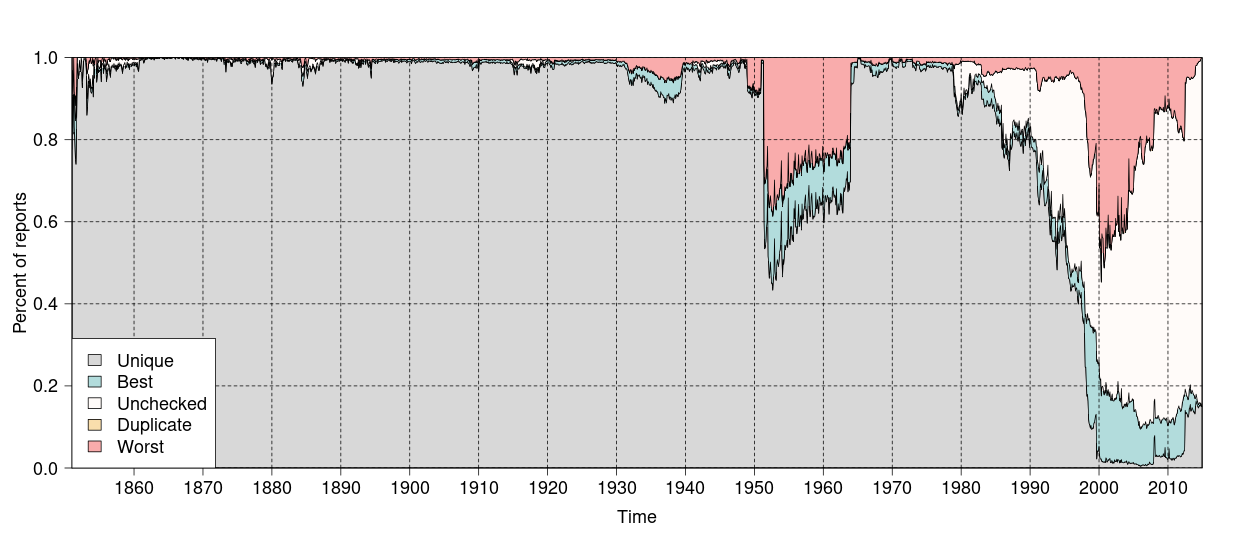
\includegraphics[width=1\textwidth]{resources/duplicate_status-ts_new.png}
    \caption{Percentage of reports flagged as unique, best duplicate, duplicate, worst duplicate or unchecked in the current data release. Reports from drifting buoys are unchecked at this stage.}
    \label{fig:dup_status}
\end{figure}

\begin{figure}[h]
    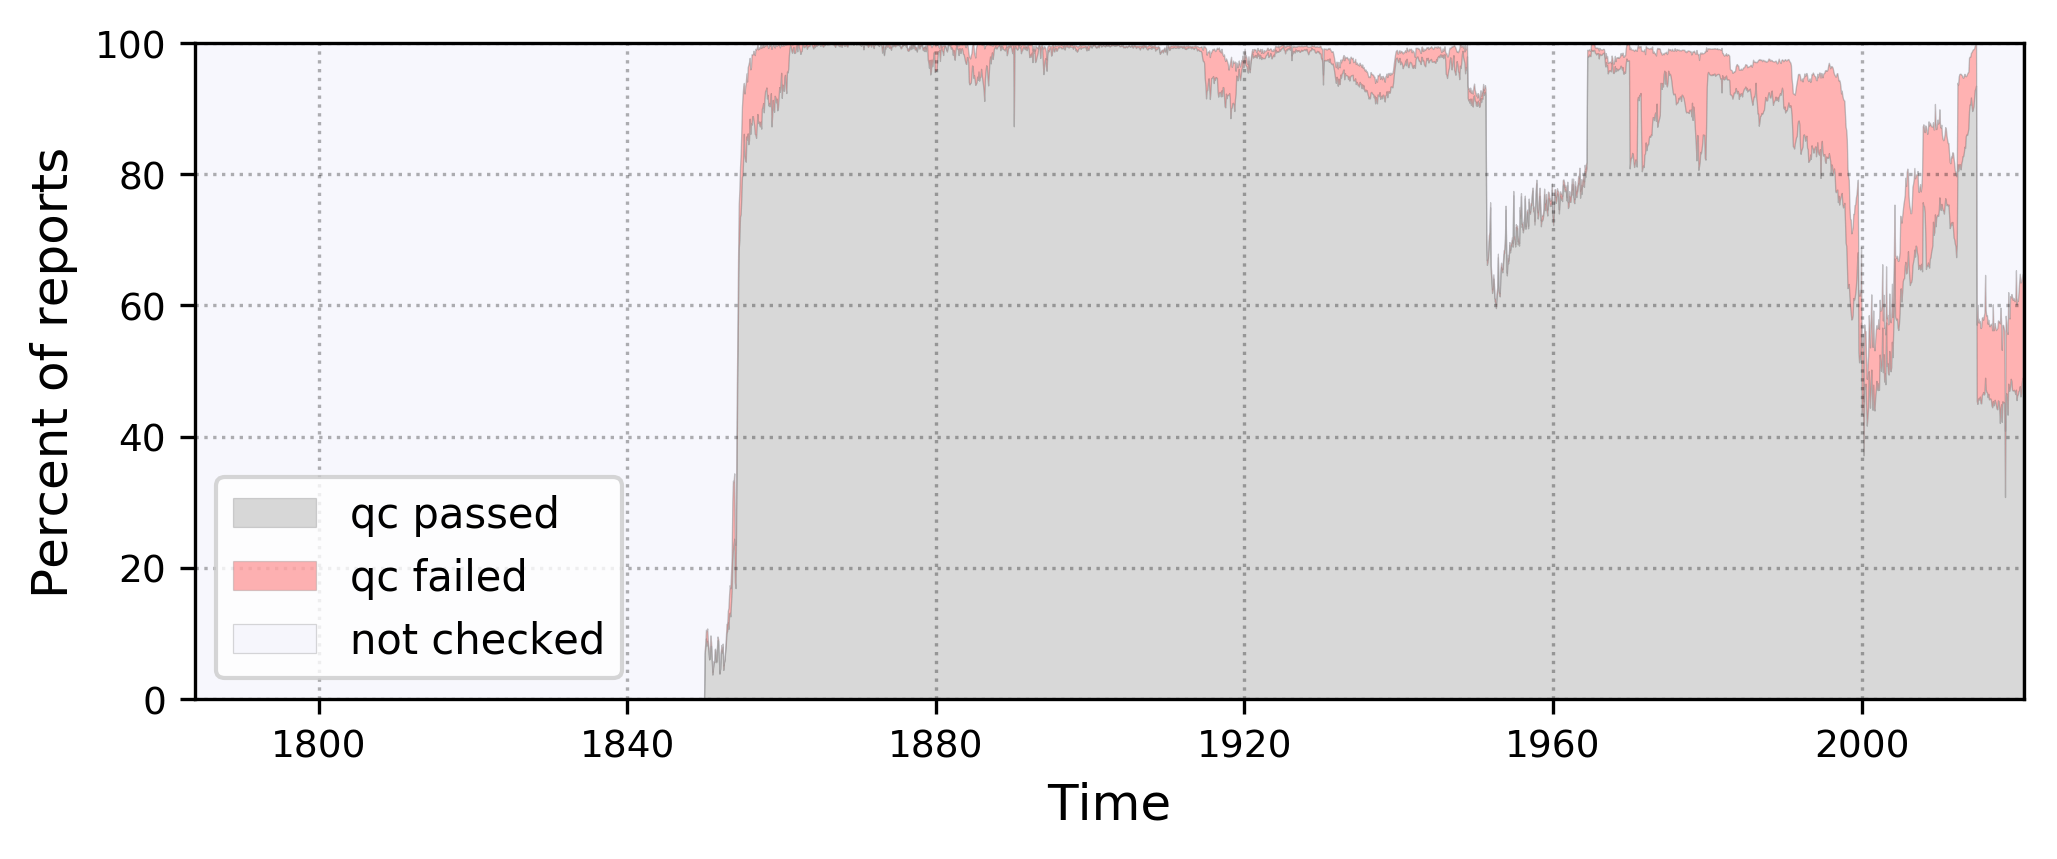
\includegraphics[width=1\textwidth]{resources/report_quality-ts.png}
    \caption{Percentage of reports flagged as unchecked, passing or failing the overall report quality check in the current data release.}
    \label{fig:report_qc}
\end{figure}
